% $Id: chapter2.tex 1790 2010-09-28 16:46:40Z jabriffa $

\chapter{Literature Review}

\section {Technologies Used}
During the entire design and implementation process, the decision was made to use the Python programming language. This choice was made originally for the ease of implementing algorithms in a scripting language like python. However, while progressing from the testing phase to the development phase, a dilemma was faced. Either to re-implement most of the progress I had made to a language that was more web and browser-based like JavaScript or, to create a hybrid of both front-end and back-end schemes. After some research online, Django was used, a high-level Python Web framework that encourages rapid development and clean, pragmatic design.

\subsection{Django Framework}
According to the official Django website, "Django is a framework that was built as a tool for front-end developers that needed a simple way to bring their ideas to life without the need of a back-end developer that handles processes such as creating and connecting the server-side with the client-side as well as the creation and handling of the system's database (Django, July 2005). Furthermore, Django is a high-level Python framework that utilizes SQLite as a relational database. Moreover, Django uses an MVT pattern similar to the more widely used MVC that frameworks like Ruby and Ruby on Rails uses.

\subsection {Atom}
Since the whole project was entirely in Django, it meant that all the code was compiled through the console. For the text and file editor, Atom was used for its familiarity and simplicity. Moreover, for testing and displaying the application, Google Chrome was used.

\section{Existing Solutions}

\subsection {Reddit Rank (Hot Sort)}
After conducting research, it was clear that one of the most popular social news aggregators currently is without a doubt, Reddit. Reddit, although it has now switched to a different ranking algorithm, since the end of 2010 but have since made their old ranking system available to the public. Their algorithm explained in the purest form takes many parameters such as the timestamp of a post, the difference between a post’s upvotes (likes) and downvotes (dislikes) and inputs those parameters in a formula that outputs a final rating that dictates a post’s position compared to others.

\begin{figure}[!htb]
 \begin{center}
	 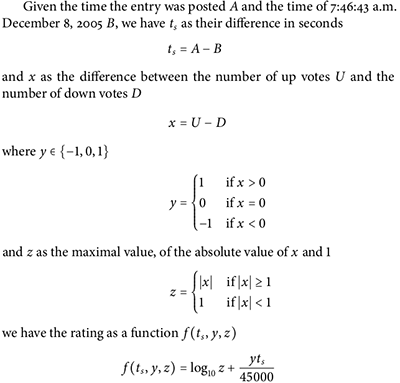
\includegraphics{Figures/reddit_rank}
 \end{center}
 \caption{Reddit Ranking Algorithm in mathematical notation}
\end{figure}


\subsubsection {Weaknesses}
\begin{itemize}
  \item An issue which is absent currently Reddit, but present in a lot of websites that take average rating as a rating attribute, is the following: Average rating works fine if you always have a ton of ratings, but suppose item 1 has 2 positive ratings and 0 negative ratings. Suppose item 2 has 100 positive ratings and 1 negative rating. This algorithm puts item two (tons of positive ratings) below item one (very few positive ratings).
\end{itemize}

\subsubsection {Conclusion}

\subsection{Hacker News Rank}
Hacker News is one of the most popular social news aggregator targeted towards developers and provides its users with mostly technology related news. Their ranking consists of three parameters, penalties, votes and age. The most impactful parameter on the formula is the penalty. The penalty's value is determined by the use of blacklisted words such as "NSA" which drops the story rapidly in the ranking. In order to keep the top stories fresh, Hacker News also issues a severe penalty on stories that reach 40 comments. The impact of a penalty can be calculated with the scoring formula since if an article gets penalty factor of 0.4, each vote will now count as 0.3. However, a factor of 0.1 is equivalent to each vote, counting 0.05. Meaning that although a penalty factor of 0.4 would drop an article 66\% faster than usual, a factor of  0.1 would drop an article by 3.6 times than normal. In outline, each item is given a ranking, and the articles are sorted according to the ranking. The simplistic way to think about ranking is the number of votes is divided by time, so more votes results in a higher ranking, but the ranking also drops over time. The votes are raised to a power less than one, while the time is raised to a power greater than one, so time has more effect than votes. Some additional penalties also may be applied to the ranking.

\begin{figure} [!htb]
  \centering
	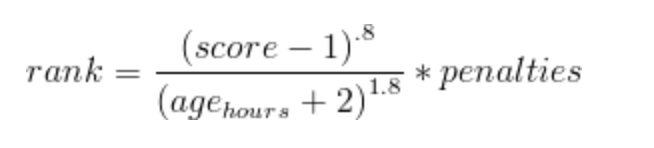
\includegraphics{Figures/hacker_news_rank}
\caption{Hacker News Algorithm in mathematical notation}
\end{figure}

\subsubsection {Weaknesses}
\begin{enumerate}
  \item Wall-clock hours penalize an article even if no one is reading (overnight, for example). A time denominated in ticks of actual activity (such as views of the 'new' page, or even upvotes-to-all-submissions) might address this.
  \item An article that misses it's audience first time through, perhaps due to (1) or a bad headline may never recover, even with a later flurry of votes far beyond what the new submissions are getting.
\end{enumerate}

\subsubsection {Conclusion}
Overall, Hacker News's algorithm is quite simple, thus making the implementation of something similar not that difficult especially since it takes into account many factors. However, there are drawbacks with using timestamps as addressed above, and a solution to this would be to use time denominated in ticks of actual activity (such as views of the 'new' page, or even upvotes-to-all-submissions) which might address this issue.
The use of penalty is an interesting concept that would make sense in a user generated content system in which there are no administrators to regulate the content.

\subsection {Wilson Confidence Sort}
The problem that the Wilson confidence score tried to resolve was, developers who need their application's users to sort things. In order to balance the proportion of positive ratings with the uncertainty of a small number of observations. The math to solve this problem was worked out in 1927 by Edwin B. Wilson(Miller, Feb. 2009). Considering only positive and negative ratings (i.e. not a 5-star scale), the lower bound on the proportion of positive ratings is given by:

\begin{figure} [!htb]
  \centering
	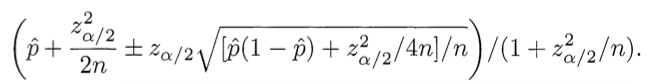
\includegraphics[scale=0.5]{Figures/wilson_confidence}
\caption{Edwin B. Wilson confidence sort in mathematical notation}
\end{figure}

\subsubsection{Conclusion}
Despite a very sought after solution to modern-day sorting, the Wilson Confidence score is to some degree. This very complicated solution only increases the efficiency of the results by a small margin. Furthermore, many problems occur in the voting system that the Wilson Confidence sort is based on. A simple example is that many people who find something mediocre will not bother to rate it at all; viewing or purchasing something and declining to rate; it contains useful information about that item's quality (Miller, Feb. 2009).

\subsection{Summary}
To summarise, most of these algorithms mentioned are tailored for their particular use or website. However, most of the existing solutions are bound by the user's interaction with the content to improve or worsen the overall score of a post. What this project is trying to propose is a system where the only interaction that is needed by the reader is their interests, after which the algorithm takes care of the rankings. Nonetheless, we can assimilate parts of existing systems that can help polish the final version of the algorithm.
